\documentclass{standalone}
\usepackage{pgfplots}
\usepackage{tikz}
\usetikzlibrary{arrows, arrows.meta, decorations.pathmorphing}

\begin{document}
    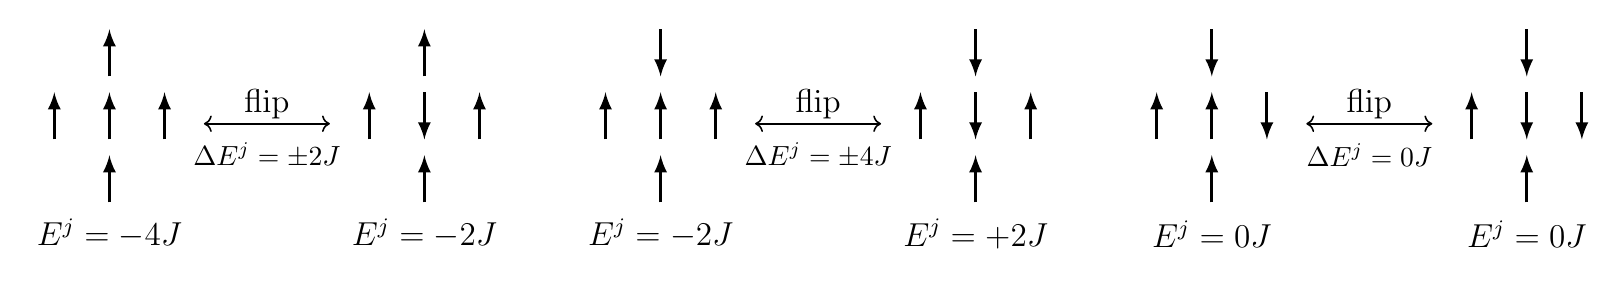
\begin{tikzpicture}[scale=1]

	    \node at (1, 0) {\large{$E^{j} = -4J$}};
	    \node at (5, 0) {\large{$E^{j} = -2J$}};

	    \node at (3, 1) {$\Delta E^{j} = \pm 2J$};

		\draw [-{latex[scale=3]}, line width = 0.4mm] (0.3,1.2) -- (0.3,1.8);        
		\draw [-{latex[scale=3]}, line width = 0.4mm] (1.0,1.2) -- (1.0,1.8);        
		\draw [-{latex[scale=3]}, line width = 0.4mm] (1.7,1.2) -- (1.7,1.8);        
		\draw [-{latex[scale=3]}, line width = 0.4mm] (1.0,2.0) -- (1.0,2.6);        
		\draw [-{latex[scale=3]}, line width = 0.4mm] (1.0,0.4) -- (1.0,1.0);

		\draw [-{latex[scale=3]}, line width = 0.4mm] (4.3,1.2) -- (4.3,1.8);        
		\draw [{latex[scale=3]}-, line width = 0.4mm] (5.0,1.2) -- (5.0,1.8);        
		\draw [-{latex[scale=3]}, line width = 0.4mm] (5.7,1.2) -- (5.7,1.8);        
		\draw [-{latex[scale=3]}, line width = 0.4mm] (5.0,2.0) -- (5.0,2.6);        
		\draw [-{latex[scale=3]}, line width = 0.4mm] (5.0,0.4) -- (5.0,1.0);

		\draw [<->, line width = 0.2mm] (2.2,1.4) -- (3.8,1.4);
		\node at (3.0, 1.65) {\large{flip}};

		%%%%%%%%%%%%%%%%%%%%%%%%%%%%%%%%%%%%%%%%%%%%%%%%%%%%%%%%%%%%%%%%%%%%%
    
	    \node at (8, 0) {\large{$E^{j} = -2J$}};
	    \node at (12, 0) {\large{$E^{j} = +2J$}};

	    \node at (10, 1) {$\Delta E^{j} = \pm 4J$};

		\draw [-{latex[scale=3]}, line width = 0.4mm] (7.3,1.2) -- (7.3,1.8);
		\draw [-{latex[scale=3]}, line width = 0.4mm] (8.0,1.2) -- (8.0,1.8);        
		\draw [-{latex[scale=3]}, line width = 0.4mm] (8.7,1.2) -- (8.7,1.8);        
		\draw [{latex[scale=3]}-, line width = 0.4mm] (8.0,2.0) -- (8.0,2.6);        
		\draw [-{latex[scale=3]}, line width = 0.4mm] (8.0,0.4) -- (8.0,1.0);

		\draw [-{latex[scale=3]}, line width = 0.4mm] (11.3,1.2) -- (11.3,1.8);        
		\draw [{latex[scale=3]}-, line width = 0.4mm] (12.0,1.2) -- (12.0,1.8);        
		\draw [-{latex[scale=3]}, line width = 0.4mm] (12.7,1.2) -- (12.7,1.8);        
		\draw [{latex[scale=3]}-, line width = 0.4mm] (12.0,2.0) -- (12.0,2.6);        
		\draw [-{latex[scale=3]}, line width = 0.4mm] (12.0,0.4) -- (12.0,1.0);

		\draw [<->, line width = 0.2mm] (9.2,1.4) -- (10.8,1.4);
		\node at (10, 1.65) {\large{flip}};

		%%%%%%%%%%%%%%%%%%%%%%%%%%%%%%%%%%%%%%%%%%%%%%%%%%%%%%%%%%%%%%%%%%%%%
    
	    \node at (15, 0) {\large{$E^{j} = 0J$}};
	    \node at (19, 0) {\large{$E^{j} = 0J$}};

	    \node at (17, 1) {$\Delta E^{j} = 0J$};

		\draw [-{latex[scale=3]}, line width = 0.4mm] (14.3,1.2) -- (14.3,1.8);        
		\draw [-{latex[scale=3]}, line width = 0.4mm] (15.0,1.2) -- (15.0,1.8);        
		\draw [{latex[scale=3]}-, line width = 0.4mm] (15.7,1.2) -- (15.7,1.8);        
		\draw [{latex[scale=3]}-, line width = 0.4mm] (15.0,2.0) -- (15.0,2.6);        
		\draw [-{latex[scale=3]}, line width = 0.4mm] (15.0,0.4) -- (15.0,1.0);

		\draw [-{latex[scale=3]}, line width = 0.4mm] (18.3,1.2) -- (18.3,1.8);        
		\draw [{latex[scale=3]}-, line width = 0.4mm] (19.0,1.2) -- (19.0,1.8);        
		\draw [{latex[scale=3]}-, line width = 0.4mm] (19.7,1.2) -- (19.7,1.8);        
		\draw [{latex[scale=3]}-, line width = 0.4mm] (19.0,2.0) -- (19.0,2.6);        
		\draw [-{latex[scale=3]}, line width = 0.4mm] (19.0,0.4) -- (19.0,1.0);

		\draw [<->, line width = 0.2mm] (16.2,1.4) -- (17.8,1.4);
		\node at (17.0, 1.65) {\large{flip}};


    \end{tikzpicture}
\end{document}